% 대한산업공학회지(JKIIE) 제출용 한글 full paper (XeLaTeX + kotex)
%   xelatex jkiie_korean.tex  (2회)
% 원칙: 기술 용어는 자연스러움을 위해 영어를 그대로 사용한다.
\documentclass[11pt,a4paper]{article}
\usepackage[margin=25mm]{geometry}
\usepackage{kotex}
\usepackage{amsmath,amssymb}
\usepackage{graphicx}
\graphicspath{{figures/}}
\usepackage{float}
\usepackage{booktabs,array}
\usepackage[font=small,labelfont=bf]{caption}
\usepackage{setspace}
\setstretch{1.28}
\usepackage[hidelinks]{hyperref}
\setlength{\parindent}{1em}

\title{\vspace{-8mm}\textbf{도착 시각(release time)과 연성 납기시각(soft due date)을 갖는\\
컴파운드 트럭 크로스도킹 스케줄링:\\
CP-SAT로 검증한 병목 유도 Iterated Local Search}}
\author{김영수\thanks{제1저자.} \quad 권상진\thanks{교신저자. Email: [지도교수 이메일 기입].}\\
\small 연세대학교 인공지능학과, 서울}
\date{}

\begin{document}
\maketitle
\vspace{-4mm}

\begin{abstract}
\noindent
컴파운드 트럭(compound truck)이 부분 하역된 뒤 특정 목적지의
출고 운송 트럭으로 전환되는 다중 도어 크로스도킹 스케줄링 문제를 다룬다.
기존 컴파운드 트럭 모델은 모든 트럭이 시각 0에 가용하다고 가정하고 총 작업완료시간
(makespan)만 최소화한다. 본 연구는 트럭별 도착 시각(release time)과 연성 납기시각
(soft due date)을 도입하여 makespan과 총 납기지연(tardiness)의 가중합을 최소화하는 문제로 확장한다. 이를 mixed-integer
program(MILP)과 CP-SAT 모형으로 정식화하고, 유효한 조합적 하한(lower bound)과
서로 겹치지 않는 train, tuning, test seed 집합을 사용한 재현 가능한 벤치마크를 제시한다. 제안 방법
VAA-GILS는 Vogel식 construction, best-improvement descent, 병목(bottleneck)을
겨냥한 guided 연산자, simulated annealing acceptance, kick restart를 결합한
iterated local search이다. CP-SAT 기준해가 존재하는 모든 실험 조건에서 VAA-GILS는
해당 CP-SAT incumbent 대비 0.1--0.6\% 이내의 목적값을 1초 미만에 얻었으며(CP-SAT는 76--376초),
소형 무(無)시간창 인스턴스에서는 증명된 최적해와 일치하였다. CP-SAT가 600초 내
실행 가능해를 찾지 못한 대형 시간창 조건에서는 비교 방법 가운데 가장 좋은 해를
제공하였다. 통제된 ablation 결과는 성능 향상이 descent, guided 연산자, restart라는 결정론적
구조에서 비롯되며, 학습 기반 연산자 선택(tabular Q-learning, transfer DQN),
학습된 초기해, 확률적 acceptance는 이 환경에서 동일 예산의 균등 연산자 선택을
능가하지 못함을 보인다.

\smallskip
\noindent\textbf{주제어:} cross-docking; compound truck; release time; soft due date;
iterated local search; constraint programming; guided local search
\end{abstract}

\section{서론}

크로스도킹은 입고 화물을 창고에 보관하지 않고 곧바로 출고 트럭으로 환적하여
재고와 리드타임을 줄이는 물류 방식이다~\cite{boysen2010,vanbelle2012}. Joo와
Kim~\cite{joo2013}이 도입하고 Shahmardan과 Sajadieh~\cite{shahmardan2020}가
발전시킨 컴파운드 트럭 변형에서는 한 대의 트럭이 두 역할을 겸한다. 여러 목적지
화물을 싣고 도착한 뒤 한 목적지의 화물은 유지하고 나머지만 \emph{부분적으로} 하역하며,
이후 해당 목적지의 나머지 화물을 적재해 출고 운송 트럭으로 출발한다. 부분 하역은 전량 하역 대비
makespan을 크게 줄이는 것으로 보고되어 LTL 통합 네트워크에서 실용적 매력이 크다.

기존 컴파운드 트럭 모델의 두 가정이 현실성을 제약한다. 첫째, 모든 트럭이 시각
0에 가용하다고 가정하지만 실제 도크에서는 트럭마다 예약 도착 시각이 다르다. 둘째,
목적함수가 순수 makespan이지만 출고 트럭의 출발은 위반 시 비용이 발생하는 due date에
묶여 있다.

도착 시각(release time), 시간창(time window), 납기지연(tardiness)은 일반 크로스도킹 스케줄링에서 이미
연구되어 왔다~\cite{vanbelle2013,assadi2016,bodnar2017,molavi2018,rijal2019,li2026}.
그러나 컴파운드 트럭 설정은 temporal constraint의 의미를 바꾼다. 컴파운드 트럭은
순수 입고 트럭도 출고 트럭도 아니다. 부분 하역 후 한 목적지의 화물을 유지하고, 해당
목적지로 들어오는 이송 화물을 기다린 뒤 비로소 출고 운송 트럭으로 출발한다. 이 부분 하역
변환은 하나의 precedence chain --- 도착 $\to$
부분 하역 $\to$ 유지 화물 $\to$ 이송 대기 $\to$ 출고 ---
을 만들고, 이 chain은 트럭들을 공유 목적지를 통해 결합한다. 따라서 release time을
추가한다고 해서 한 트럭의 시작 시각만 늦어지는 것은 아니다. 늦은 도착은 해당 트럭의
이송 화물에 의존하는 모든 출고 운송 트럭으로 전파되고, soft due date는 이 연쇄 지연을
tardiness 비용으로 바꾼다. 본 연구의 기여는 이 상호작용 --- 알려진 release time과
soft due date가 부분 하역 후 출고 운송 트럭으로 전환되는 과정과 결합되는 방식 --- 을 정식화하고 분석하는
것이며, 저자가 아는 한 이 결합은 이전에 모형화된 바 없다.

본 논문의 기여는 세 가지다. 첫째, 독립적인 스케줄 평가기와 일치하는 big-$M$ MILP
및 reified CP-SAT 정식화와, 목적함수에 대한 유효 조합 하한을 제시한다. 둘째, 기존
VAA construction과 generic neighborhood에 full best-improvement descent, 병목 유도
연산자, kick restart를 더한 VAA-GILS를 제안한다. 셋째, 통제된 ablation으로 성능이
탐색 엔진에서 비롯되는지 학습 기반 연산자 선택에서 비롯되는지를 구분하며, 후자는
동일 예산의 균등 선택 방식을 능가하지 못함을 보인다. 이 결과는 강한 탐색 엔진
안에서 학습 기반 선택기를 평가할 때 동일 예산의 균등 선택 방식이 필요함을
시사한다.

\section{관련 연구}

\textbf{시간 제약이 있는 크로스도킹 스케줄링.} Boysen과 Fliedner~\cite{boysen2010}는
도크 스케줄링 문제를 분류하였고, Van Belle 등~\cite{vanbelle2012}은 분야를
조망하였다. 여러 결정론적 모형이 기존 입고·출고 트럭에 대해 시간
제약을 이미 반영한다. Van Belle 등~\cite{vanbelle2013}은 다중 도어·time window·
tardiness를, Assadi와 Bagheri~\cite{assadi2016}는 ready time과 outbound
earliness/tardiness를, Bodnar 등~\cite{bodnar2017}은 time window와 mixed-service
door를 다룬다. Molavi 등~\cite{molavi2018}은 hard due date를, Rijal
등~\cite{rijal2019}은 truck scheduling과 door assignment의 통합을 다룬다. 이들은
release/due date가 새롭지 않음을 보이나, 입고·출고 트럭을 구분하며 부분
하역 후 출고 운송 트럭으로 전환되는 트럭을 모형화하지 않는다.

\textbf{불확실·불완전 도착 정보.} 도착 불확실성은 별도의 흐름이다. Konur와
Golias는 bounded arrival window~\cite{konur2013}와 unknown arrival 하의 cost-stable
schedule~\cite{konurcost2013}을 다룬다. Larbi 등~\cite{larbi2011}은 도착 정보의
full/partial/absent를 구분하고, Ladier와 Alpan~\cite{ladier2016}은 time window
하의 robust schedule을, Xi 등~\cite{xi2020}은 two-stage conflict robust
optimization을 제시한다. 본 모형은 결정론적이며 각 release time은 스케줄 구성
시점에 알려져 있다. 따라서 이들 불확실성 모형은 본 모형을 직접 대체하기보다 향후
자연스럽게 확장할 수 있는 연구 방향에 해당한다.

\textbf{가장 유사한 문제와 학습형 메타휴리스틱.} Li 등~\cite{li2026}은 mixed
service mode door와 time window의 통합 트럭 배정·스케줄링을 Q-learning 기반 ALNS로
푼다. 그 유연성은 도어 수준에 있고 트럭은 순수 입고·출고 트럭인 반면, 본 문제의
유연성은 트럭 수준(컴파운드 트럭, 도어 간 직접 이송)에 있다. 한편 학습 기반
operator selection이 메타휴리스틱을 개선한다는 보고가 많으나, 본 연구는 강한 지역
탐색을 갖춘 뒤에는 learned selector의 이득이 작다는 통제된 반례를 더한다.

\section{문제 정의}

\subsection{기본 모델}
$I$, $F$, $D$, $K$, $M$을 각각 컴파운드 트럭, 출고 트럭, 목적지, 상품 종류,
도어의 집합이라 하고 $|I|+|F|=|D|$, $|I|\le|M|$이라 하자. 컴파운드 트럭 $i$는
목적지 $d$행 상품 $k$를 $f_{idk}$ 단위 싣는다. 단위 처리시간 $t_k$, 도어
$m,n$ 간 배치 이송시간 $t_{mn}$, 트럭 $i$의 진입·출차 전환시간
$DE_i,DL_i$에 대해 $h_{id}=\sum_k f_{idk}t_k$, $H_i=\sum_d h_{id}$로 둔다. 각
컴파운드 트럭은 유지할 목적지 하나와 도어 하나를(도어당 컴파운드 최대 1대), 각
출고 트럭은 남은 목적지 하나와 도어를 고르며, 같은 도어의 출고 트럭은
작업 순서를 정한다. 각 목적지에는 정확히 하나의 운송 트럭이 배정된다.

시간 계산은 스케줄 평가기 규칙을 따른다. 컴파운드 트럭 $i$(목적지 $d$ 유지)의 하역은
$r_i+DE_i+\sum_{d'\ne d}h_{id'}$에 끝난다. 운송 트럭은 화물을 보내는 모든 트럭의 하역과
도어 간 이송이 끝나야 적재할 수 있다. 출고 운송 트럭 $f$는 추가로 자신의
release와 도어의 선행 점유가 끝나는 시점에 도어 작업을 시작하여
$S_f=\max(\text{door available},\ \text{destination ready},\ r_f)$이며, 이후
진입($DE_f$), 적재, 출차($DL_f$)를 차례로 수행하므로 완료 시각은
$S_f+DE_f+L_d+DL_f$이다. 즉 $S_f$는 적재 시작이 아니라 도어 작업 시작 시각이고,
적재는 $S_f+DE_f$에 시작한다. makespan $\tau=C_{\max}$는 최대 완료 시각이다.

\subsection{Mixed-integer 정식화}
이진 변수 $x_{idm}$은 컴파운드 트럭 $i\in I$를 유지 목적지 $d$·도어 $m$에,
$z_{fdm}$은 출고 트럭 $f\in F$를 배정한다. $X_{im}=\sum_d x_{idm}$,
$Z_{fm}=\sum_d z_{fdm}$, $Z_{fd}=\sum_m z_{fdm}$로 두고, $b_{fgm}$은 도어 $m$에서
$f$가 $g$에 선행하면 1이다. 연속 변수 $U_i,C_i,S_f,C_f,C_{\max}$는 각각 컴파운드
하역 완료, 컴파운드 완료, 출고 도어 작업 시작, 출고 완료, makespan이다.
$L_{id}=\sum_{j\ne i}h_{jd}$, $L_d=\sum_i h_{id}$, $B$는 유효한 horizon 상한이다.

\begin{align}
&\textstyle\sum_{d,m}x_{idm}=1\ \ \forall i,\qquad \sum_{d,m}z_{fdm}=1\ \ \forall f, \\
&\textstyle\sum_{i,m}x_{idm}+\sum_{f,m}z_{fdm}=1\ \ \forall d,\qquad \sum_{i,d}x_{idm}\le1\ \ \forall m.
\end{align}
컴파운드 타이밍과 incoming-transfer precedence는
\begin{align}
U_i&=r_i+DE_i+H_i-\textstyle\sum_{d,m}h_{id}x_{idm}\quad\forall i,\\
C_i&\ge U_i+L_{id}+DL_i-B(1-x_{idm})\quad\forall i,d,m,\\
C_i&\ge U_j+t_{nm}+L_{id}+DL_i-B(2-x_{idm}-X_{jn})
\end{align}
로, 모든 $i,d,m,n$과 $\sum_k f_{jdk}>0$인 기여 $j\ne i$에 대해 성립한다. 출고
운송 트럭에 대해서는
\begin{align}
S_f&\ge r_f\quad\forall f,\\
C_f&\ge S_f+DE_f+L_d+DL_f-B(1-Z_{fd})\quad\forall f,d,\\
S_f&\ge U_i+t_{nm}-B(2-z_{fdm}-X_{in}),\\
S_f&\ge C_i-B(2-Z_{fm}-X_{im})\quad\forall f,i,m.
\end{align}
같은 도어 $m$의 출고 트럭 쌍 $f<g$에 대해 $b_{fgm}+b_{gfm}\ge Z_{fm}+Z_{gm}-1$,
$b_{fgm}\le Z_{fm}$, $b_{fgm}\le Z_{gm}$이며 non-overlap은
\begin{equation}
S_g\ge C_f-B(1-b_{fgm}),\qquad S_f\ge C_g-B(1-b_{gfm}).
\end{equation}
끝으로 $C_{\max}\ge C_i\ \forall i$, $C_{\max}\ge C_f\ \forall f$. CP-SAT 모형은
big-$M$ disjunction을 enforcement literal로 대체하고 시간을 0.01 단위로
정수화하며, 모든 배정을 고정하면 독립 evaluator의 완료 시각이 재현되어 model
fidelity가 확인된다.

\subsection{시간창 확장과 목적함수}
각 트럭 $q\in I\cup F$는 release time $r_q\ge0$과 연성 납기시각 $\bar d_q$를 갖고
$T_q\ge\max\{0,C_q-\bar d_q\}$이다. 목적함수는
\begin{equation}
\min\ J=C_{\max}+\lambda\sum_{q\in I\cup F}T_q,\qquad \lambda=1.
\label{eq:obj}
\end{equation}
$r_q=0$, $\bar d_q=\infty$이면 기존 makespan 모델로 환원된다. CP-SAT는 incumbent와
증명된 하한을 함께 반환하며, 하한과 일치가 증명될 때에만 최적으로 부른다.

\subsection{조합적 하한}
정확해법이 제공하는 하한이 약한 실험 조건에서 gap을 보고하기 위해 도어 경합을 완화한 두 유효 하한을
사용한다. 컴파운드 트럭 $i$(목적지 $d$ 유지)의 최속 완료와 출고 트럭 $f$의 최속
완료는
\begin{align}
EF_i&=r_i+DE_i+\min_{d\in D}\Big(H_i-h_{id}+\textstyle\sum_{j\in I\setminus\{i\}}h_{jd}\Big)+DL_i,\\
EF_f&=r_f+DE_f+\min_{d\in D}\textstyle\sum_{j\in I}h_{jd}+DL_f.
\end{align}
critical-chain 하한은 $LB_{\mathrm{cc}}=\max_{q\in I\cup F}EF_q$이다. door-area
하한은 각 트럭의 최소 도어 점유
\[
o_i=DE_i+\Big(H_i-\max_d h_{id}\Big)+\min_d\textstyle\sum_{j\in I\setminus\{i\}}h_{jd}+DL_i,\quad
o_f=DE_f+\min_d\textstyle\sum_{j\in I}h_{jd}+DL_f
\]
을 도어 수로 나눈 $LB_{\mathrm{da}}=\frac1{|M|}\big(\sum_i o_i+\sum_f o_f\big)$이다.
둘 다 제약을 완화하므로 $LB_\tau=\max\{LB_{\mathrm{cc}},LB_{\mathrm{da}}\}$는
makespan의 유효 하한이며, 각 $EF_q$가 $C_q$의 하한이므로
$LB_T=\sum_{q:\bar d_q<\infty}\max\{0,EF_q-\bar d_q\}$이고
$LB_J=LB_\tau+\lambda LB_T$는 식~\eqref{eq:obj}의 유효 하한이다.

\section{VAA-GILS}

VAA-GILS는 iterated local search의 구현체로, 연산자 내부 sampling과 acceptance를
제외하면 결정론적이다.

\textbf{초기해 구성.} VAA는 Vogel식 regret으로 유지 목적지를 정하고, 완료 시각
우선순위에 따라 출고 목적지를 배정한 뒤 완료 예정 시각이 가장 이른 도어에 삽입한다.
모든 완료 예정 시각 계산에는 release time을 반영한다.

\textbf{Descent.} 세 무브군(출고 트럭 재배치, 컴파운드 트럭의 도어 교환/빈 도어 이동, 두
트럭 목적지 스왑)에 대한 best-improvement 지역탐색으로, local optimum에서
종료하며 초기해·모든 신규 incumbent·최종해에 적용한다.

\textbf{반복 탐색.} 1{,}000회 반복한다. 선택 정책이 연산자 하나를 뽑아
현재 해에서 후보를 생성하고, 후보가 전역 best를 개선하면 descent를 적용해
incumbent를 갱신한다. acceptance는 초기 온도 $T_0=\max\{1,0.05\,J(s_0)\}$, 기하
냉각 $T\leftarrow0.995\,T$의 simulated annealing이다. 30회 연속 개선이 없으면 현재 최선해에서
random kick 3회로 재시작하고 $T\leftarrow\max\{T,0.02\,J(s^*)\}$로 reheat한다.

\textbf{Operator pool.} generic neighborhood 7종에, 현재 병목을 먼저 식별한 뒤 그
주변을 best-of로 탐색하는 guided 연산자 4종을 더한다: (g1) critical door의 마지막
출고 트럭을 최선 도어·위치로 재배치, (g2) critical 트럭의 목적지를 전 트럭과
대조해 최선 스왑, (g3)/(g4) most tardy 트럭 기준의 동일 무브(tardy인 트럭이 없으면
g1/g2로 fallback). 고속 증분 evaluator(평가당 수십 $\mu$s)가 descent와 guided 무브를
저렴하게 만든다.

\textbf{선택 정책과 원 모델의 비교.} 선택 정책은 교체할 수 있으며 기본값은
균등 무작위 선택이다. 학습 정책(SA-RL5의 tabular Q-learning, 규모 불변 피처로
오프라인 학습한 transfer DQN)는 ablation 목적으로만 평가하며 제안 방법의 일부가
아니다. 원 모델 SA-RL5는 RL이 단일 무브를 고르고 SA accept/reject로 스텝이 끝나는
\emph{순수} simulated annealing인 반면, VAA-GILS는 그 한 연산자 스텝을 iterated
local search 안에 넣고 guided 연산자, 개선 무브마다의 full descent, kick
restart를 더한다. 가장 중요한 차이는 개선 무브 이후의 descent이며, ablation은
이것이 품질 이득의 대부분을 설명함을 보인다. 표~\ref{tab:base}가 두 방법의 구조적
차이를 요약한다.

\begin{table}[H]\centering
\caption{원 모델 SA-RL5와 VAA-GILS의 구조 비교.}
\label{tab:base}\small
\begin{tabular}{@{}p{0.24\columnwidth}p{0.33\columnwidth}p{0.33\columnwidth}@{}}
\toprule
항목 & SA-RL5 (base) & VAA-GILS (제안) \\
\midrule
전체 틀 & 순수 simulated annealing & iterated local search (SA는 acceptance만) \\
반복당 연산자 & 1개 & 1개 (동일) \\
연산자 pool & 이웃 7종 & 그 7종 + guided 4종 \\
연산자 선택 & online Q-learning/roulette & uniform random (학습은 ablation 전용) \\
개선 무브 이후 & 없음(SA step이 전부) & full best-improvement descent \\
정체 처리 & 없음 & kick restart + reheat \\
acceptance & SA(Metropolis) & SA(Metropolis; ablation상 생략 가능) \\
목적함수 & makespan & makespan $+\lambda\cdot$ tardiness \\
\bottomrule
\end{tabular}
\end{table}

\section{실험 설계}
세 규모 $(|I|,|D|,|M|)$: S $(6,9,6)$, M $(12,18,12)$, L $(20,30,20)$, 컴파운드
비율 $2/3$을 사용한다. flow는 상품 3종에 대해 $[0,20]$의 균등 정수,
$t_k\sim U[1,5]$, 도어는 $100\times100$ 랜덤 배치이다. 시간창 수준은
none/medium/tight이며 medium/tight에서 $r\sim U[0,\rho H]$, $\bar d=r+\delta H$,
$(\rho,\delta)=(0.25,0.60),(0.50,0.35)$이다.

seed는 서로소인 train/tuning/test 풀로 분리한다. 주 해품질 비교(표~\ref{tab:main})는
셀당 test 인스턴스 20개 $\times$ replication 5회를 사용하고, 통제된 ablation은
동일예산·동일구조 분해이므로 원래의 5-인스턴스 설계를 유지한다. 인스턴스별로
replication을 평균한 뒤 짝지은 인스턴스 평균에 양측 Wilcoxon signed-rank test를
적용한다. GILS는 1{,}000회 반복한다. CP-SAT는 인스턴스당 1회, 8 thread로 S
300초(5개), M/L 600초(셀당 2개) 실행하며 S-none 5개만 최적이 증명된다. 주 지표는
모든 방법과 예산 및 CP-SAT 결과를 포함하여 관측된 최선해에 대한 인스턴스별 gap
$\Delta_{bo}$이다.

\section{실험 결과}
\subsection{해 품질}
표~\ref{tab:main}이 20-인스턴스 test 결과를 요약한다. 평균목적값·$\Delta_{bo}$는
20-인스턴스 기준이고, vs CP-SAT는 CP-SAT 기준해가 있는 부분집합(S 셀 5개, M-none 2개)만이며
S-none만 최적이 증명된다. CP-SAT 기준해가 있는 모든 실험 조건에서 GILS는 이에 근접한다
(vs CP-SAT 0.1--0.6\% 이내). 기본(default) selector인 uniform 기준으로, GILS는 VAA를
평균 2.65\%($n=180$, $p<10^{-4}$), SA-RL5를 1.38\%($n=60$, $p<10^{-4}$) 능가한다.
GILS의 평균 실행 시간은 S/M/L에서 0.11, 0.52, 2.3초, CP-SAT는 76, 237, 376초이다.

\begin{table}[t]\centering
\caption{20-인스턴스 test 결과. $\Delta_{bo}$는 관측된 최선해 대비 평균 gap.
vs CP-SAT는 CP-SAT 기준해가 있는 부분집합(S-none은 증명된 최적).}
\label{tab:main}\small
\begin{tabular}{@{}llrrr@{}}
\toprule
셀 & 방법 & 평균목적값$\pm$표준편차 & $\Delta_{bo}$(\%) & vs CP-SAT(\%)\\
\midrule
S-none & VAA & $1497.5\pm400.3$ & 6.60 & $+6.49$\\
 & Paper-SA-RL5 & $1423.3\pm383.6$ & 1.03 & $+1.21$\\
 & GILS-uniform & $1411.8\pm382.7$ & 0.16 & $+0.21$\\
 & GILS-tabular & $1412.9\pm381.3$ & 0.28 & $+0.33$\\
 & GILS-DQN & $1416.1\pm382.4$ & 0.51 & $+0.75$\\
S-medium & VAA & $5447.5\pm1468.9$ & 3.89 & $+3.33$\\
 & GILS-uniform & $5255.7\pm1413.3$ & 0.08 & $+0.11$\\
 & GILS-tabular & $5259.1\pm1412.3$ & 0.15 & $+0.18$\\
 & GILS-DQN & $5270.8\pm1415.3$ & 0.38 & $+0.55$\\
S-tight & VAA & $9276.8\pm2387.6$ & 2.90 & $+2.17$\\
 & GILS-uniform & $9010.8\pm2206.1$ & 0.09 & $+0.21$\\
 & GILS-tabular & $9011.9\pm2206.7$ & 0.11 & $+0.17$\\
 & GILS-DQN & $9022.0\pm2205.3$ & 0.23 & $+0.34$\\
M-none & VAA & $3030.9\pm903.6$ & 3.73 & $+4.80$\\
 & Paper-SA-RL5 & $2976.4\pm864.4$ & 1.86 & $+0.99$\\
 & GILS-uniform & $2928.9\pm842.6$ & 0.29 & $+0.13$\\
 & GILS-tabular & $2932.1\pm846.3$ & 0.37 & $+0.11$\\
 & GILS-DQN & $2932.5\pm845.5$ & 0.40 & $+0.19$\\
M-medium & VAA & $23025.5\pm4075.4$ & 2.56 & ---\\
 & GILS-uniform & $22526.4\pm3960.5$ & 0.29 & ---\\
 & GILS-tabular & $22515.5\pm3964.0$ & 0.24 & ---\\
 & GILS-DQN & $22540.3\pm3956.4$ & 0.36 & ---\\
M-tight & VAA & $38903.7\pm11283.5$ & 1.25 & ---\\
 & GILS-uniform & $38528.0\pm11078.0$ & 0.19 & ---\\
 & GILS-tabular & $38512.1\pm11059.5$ & 0.16 & ---\\
 & GILS-DQN & $38543.6\pm11077.6$ & 0.24 & ---\\
L-none & VAA & $5492.3\pm1482.2$ & 2.21 & ---\\
 & Paper-SA-RL5 & $5479.7\pm1449.5$ & 1.97 & ---\\
 & GILS-uniform & $5388.4\pm1427.3$ & 0.27 & ---\\
 & GILS-tabular & $5385.5\pm1424.6$ & 0.22 & ---\\
 & GILS-DQN & $5386.1\pm1425.2$ & 0.23 & ---\\
L-medium & VAA & $55611.1\pm18087.3$ & 1.52 & ---\\
 & GILS-uniform & $54846.4\pm17523.5$ & 0.10 & ---\\
 & GILS-tabular & $54833.4\pm17526.8$ & 0.07 & ---\\
 & GILS-DQN & $54848.8\pm17522.9$ & 0.11 & ---\\
L-tight & VAA & $119671.9\pm32475.3$ & 0.77 & ---\\
 & GILS-uniform & $118901.4\pm31781.1$ & 0.08 & ---\\
 & GILS-tabular & $118865.6\pm31788.4$ & 0.05 & ---\\
 & GILS-DQN & $118888.8\pm31789.1$ & 0.07 & ---\\
\bottomrule
\end{tabular}
\end{table}

\subsection{성능은 어디에서 오는가}
세 가지 통제된 ablation(예산 1{,}000회 고정)으로 엔진을 분해한다.

\textbf{Operator pool.} selection을 uniform으로 고정하고 pool만 generic(7)/
critical(+g1,g2)/full(+g3,g4)로 바꾸면 $\Delta_{bo}$가 9개 셀 전부에서
generic $\ge$ critical $\ge$ full로 단조 감소한다(그림~\ref{fig:op}). 짝지은
Wilcoxon(표~\ref{tab:b1})은 유도 연산자가 목적값을 일관되게·유의하게 낮춤을
보인다.

\begin{table}[H]\centering
\caption{Operator-pool ablation(양측 Wilcoxon; $+$평균 = 풍부한 pool이 우세).}
\label{tab:b1}\small
\begin{tabular}{@{}lrrl@{}}
\toprule
대비 & $n$ & 개선(\%p) & $p$\\
\midrule
generic $\to$ critical (g1,g2 추가) & 136 & $+0.114$ & $<10^{-4}$\\
critical $\to$ full (g3,g4 추가) & 172 & $+0.048$ & $<10^{-4}$\\
generic $\to$ full (전체 유도) & 166 & $+0.161$ & $<10^{-4}$\\
\bottomrule
\end{tabular}
\end{table}

\begin{figure}[H]\centering
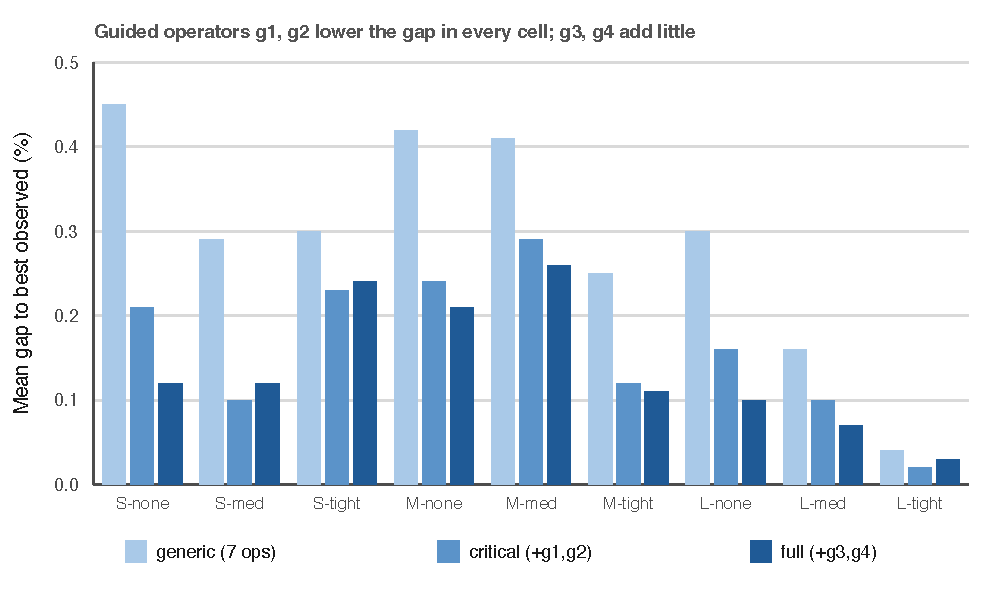
\includegraphics[width=0.82\columnwidth]{fig2_operator_pool.pdf}
\caption{operator pool별 관측된 최선해 대비 gap.}\label{fig:op}
\end{figure}

\textbf{Engine components.} pool을 full, selection을 uniform으로 고정하고 컴포넌트를
하나씩 제거하면(표~\ref{tab:b2}), best-improvement descent의 기여가 가장 크고 kick
restart가 그다음이며, VAA 초기해는 통계적으로 유의하지 않고 확률적 acceptance는
제거해도 목적값이 나빠지지 않는다(그림~\ref{fig:comp}).

\begin{table}[H]\centering
\caption{Engine-component ablation(leave-one-out; 제거 시 상대 목적값 악화율).}
\label{tab:b2}\small
\begin{tabular}{@{}lrrl@{}}
\toprule
제거 컴포넌트 & $n$ & 악화(\%p) & $p$\\
\midrule
best-improvement descent & 45 & $+0.156$ & $<10^{-4}$\\
kick restart & 43 & $+0.069$ & $<10^{-4}$\\
VAA initial solution & 45 & $+0.022$ & 0.114\\
stochastic acceptance & 45 & $-0.026$ & 0.0014\\
\bottomrule
\end{tabular}
\end{table}

\begin{figure}[H]\centering
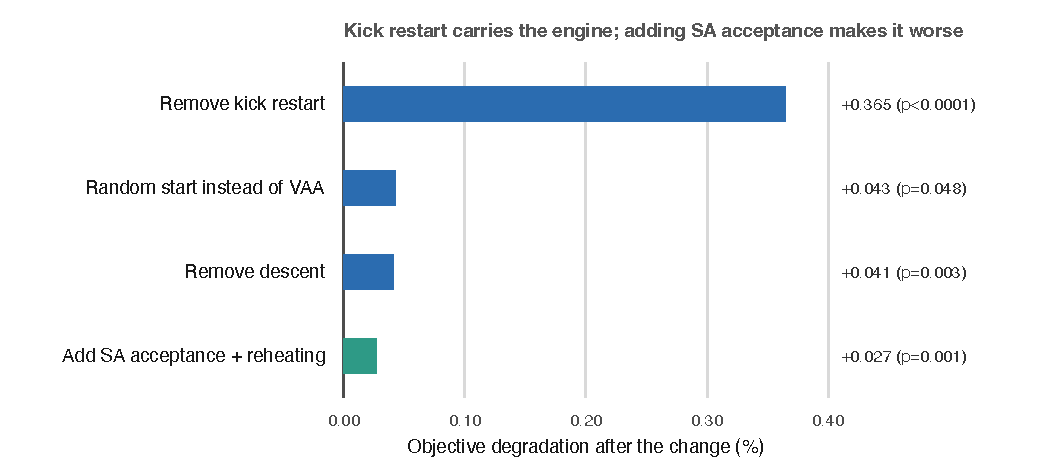
\includegraphics[width=0.82\columnwidth]{fig3_component_ablation.pdf}
\caption{컴포넌트 제거 시 목적값 악화율.}\label{fig:comp}
\end{figure}

\textbf{Learned operator selection.} pool과 컴포넌트를 full로 고정하고 selection만
바꾸면(표~\ref{tab:sel}), 어떤 learned policy도 uniform을 실용적으로 능가하지
못한다. 예산 50--3{,}000회에서 uniform은 $0.47\to0.16\%$, tabular는
$0.56\to0.09\%$, DQN은 $0.56\to0.26\%$로 움직이며, 방향은 예산에 따라 뒤집힌다
(그림~\ref{fig:sel}). 이러한 부정적 결과는 무시간창 셀만으로도 성립하므로 시간창
확장 때문에 나타난 결과가 아니다.

\begin{table}[H]\centering
\caption{1{,}000회에서의 selection 효과(양측 Wilcoxon; 양의 평균 = 앞 방법 우세).}
\label{tab:sel}\small
\begin{tabular}{@{}lrrl@{}}
\toprule
비교 & 평균차(\%p) & $p$ & 판정\\
\midrule
tabular vs uniform & $-0.01$ & 0.150 & 차이 없음\\
tabular vs DQN & $+0.10$ & $<10^{-4}$ & DQN 열세\\
uniform vs DQN & $+0.11$ & $<10^{-4}$ & DQN 열세\\
\bottomrule
\end{tabular}
\end{table}

\begin{figure}[H]\centering
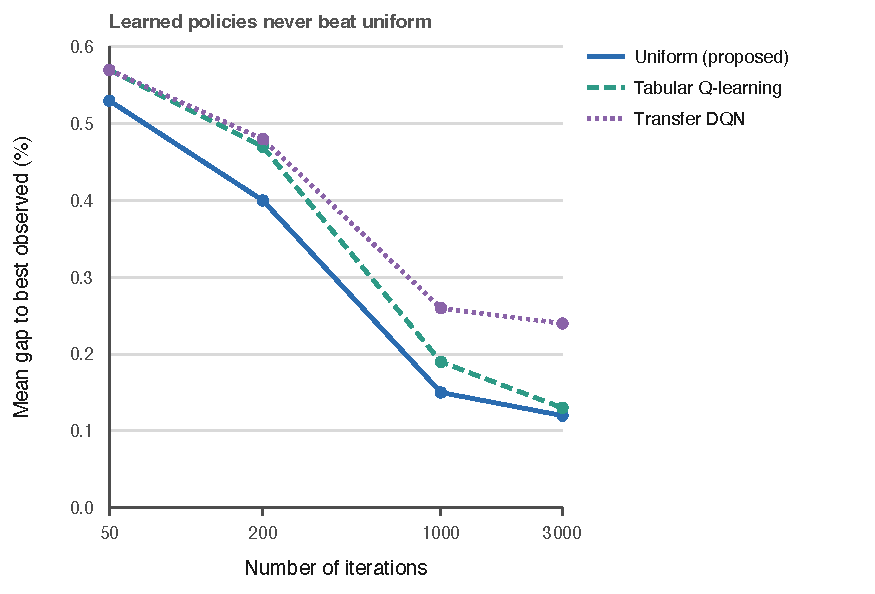
\includegraphics[width=0.72\textwidth]{fig1_selector_budget.pdf}
\caption{iteration budget에 따른 관측된 최선해 대비 gap.}\label{fig:sel}
\end{figure}

\subsection{Tardiness-weight 민감도}
식~\eqref{eq:obj}이 시간 단위 성분 둘을 합치므로 tuning 풀에서
$\lambda\in\{0,0.25,0.5,1,2,4,8\}$을 스윕한다. 물리적 makespan과 총 tardiness를
인스턴스별로 min--max 정규화해 평균한다(그림~\ref{fig:lam}). tardiness 감소의
대부분은 $\lambda=0$에서 $1$ 사이에서 일어나고 이후에는 그 폭이 줄어든다. 전체 스윕 구간에서 평균
makespan은 약 1\% 상승, 평균 tardiness는 2--3\% 하락한다. $\lambda=1$을 채택한다:
완만한 makespan 비용으로 tardiness가 거의 최소에 이르고 두 시간 성분에 동일
가중을 준다. 이 스윕은 test가 아닌 tuning 인스턴스를 사용한 설계 정당화이다.

\begin{figure}[H]\centering
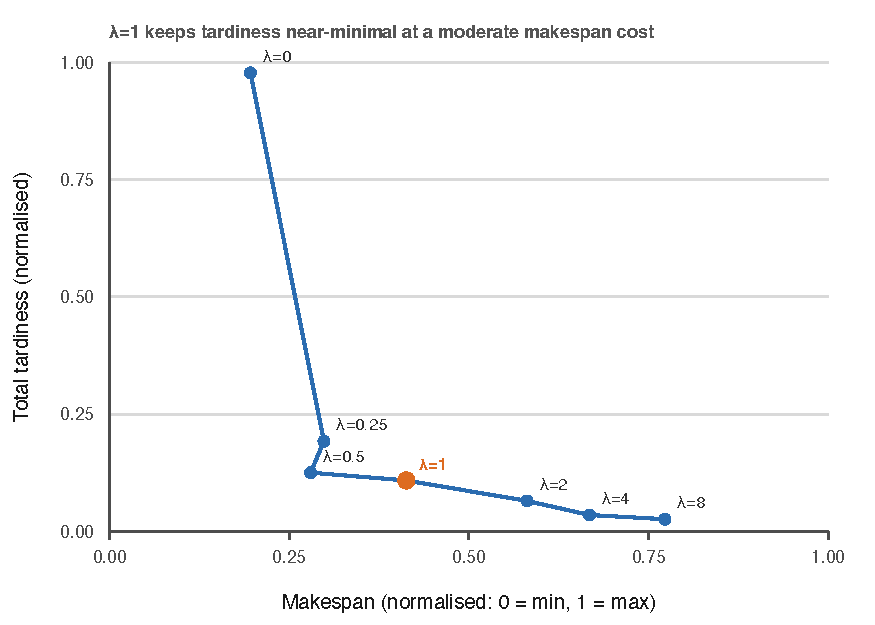
\includegraphics[width=0.72\textwidth]{fig4_lambda_tradeoff.pdf}
\caption{tuning 인스턴스에서의 정규화된 makespan--tardiness trade-off.}\label{fig:lam}
\end{figure}

\section{논의}
selector 결과는 본 탐색 과정 안에서 해석해야 한다. 후보 평가가 수십 $\mu$s로
저렴하고, 모든 신규 incumbent 뒤에 결정론적 descent가 따른다. 같은 basin에
들어간 두 실행은 선행 무브가 달라도 같은 해로 수렴할 수 있으며, budget 곡선은 이
수렴이 대부분의 test 인스턴스에서 1{,}000회 이전에 일어남을 시사한다. 같은
이유로 SA acceptance와 reheating은 기저 SA-RL5 framework와의 comparability를 위해
유지하였으나, ablation은 본 설정에서 이들이 해 품질에 필수적이지 않음을 보인다.

정책이 예측할 정보도 적다. 인스턴스는 정적이고 모든 release는 최적화 전에 알려져
있다. 이는 도착 정보가 시간의 흐름에 따라 공개되는 online dock control이나 개별 무브의 평가 비용이
비싼 simulation 모형과 다르며, 그런 환경에서는 learned selection의 역할이 커질 수
있다. 본 결과가 뒷받침하는 바는 제한적이다. 즉, learned selector는 동일한 엔진과 동일한
예산에서 uniform sampling과 비교되어야 하며, 그 통제가 없으면 descent·restart·강한
무브군의 이득이 정책 자체의 것으로 잘못 귀속될 수 있다.

\section{결론}
본 연구는 부분 하역 컴파운드 트럭 스케줄링에 release time과 연성 납기시각을
도입하고, MILP·CP-SAT 정식화와 유효 하한으로 휴리스틱 해를 검증하였다. CP-SAT
기준해가 있는 실험 조건에서 VAA-GILS의 목적값은 해당 incumbent 대비 1\% 미만이었고(소형은 증명된
최적), 대형 시간창 조건에서는 수 초 안에 비교 방법 가운데 가장 좋은 해를 제공하였다.
ablation은 성능이 best-improvement descent, guided 무브, restart라는 결정론적
구조에서 비롯되며, 학습 기반 연산자 선택·학습된 초기해·확률적 acceptance는 이
환경에서 실용적 이득을 주지 않음을 보였다. 향후에는 도착 정보가 실시간으로 공개되는 동적
문제, 대형 시간창 조건을 위한 더 강한 하한, 산업 데이터를 활용한 사례 연구가 필요하다.

\appendix
\section{Transfer DQN 구현 세부}
transfer DQN은 매 반복 11개 연산자 pool에서 하나를 고른다. Q-network는 27차원 규모
불변 상태를 연산자별 Q값으로 사상하는 MLP로, 64 unit의 hidden layer 2개와 ReLU를
쓴다. 학습은 용량 100{,}000의 replay buffer를 사용하며, 500 transition warm-up 후
매 step 1회 gradient step으로 Huber(smooth-$L_1$) temporal-difference loss를 Adam
(learning rate $10^{-3}$, discount $\gamma=0.9$)으로 최소화한다. mini-batch는 64,
target network는 500 step마다 동기화한다. reward는 shaped signal(신규 incumbent 2,
비악화 1, 그 외 0)이다. agent는 \emph{train} 풀(S/M 규모, 모든 flow·시간창 조건)에서 500회
실행으로 오프라인 학습($\varepsilon$-greedy) 후, \emph{test} 인스턴스에 zero-shot
($\varepsilon=0$, 갱신 없음)으로 적용한다. 결과가 uniform 대비 개선이 없다는
것이므로, 재현·강화가 가능하도록 network·학습 스크립트·seed를 공개한다.

\section*{생성형 AI 사용 명시}
원고 준비 과정에서 저자들은 언어 교정, 원고 구성, 참고문헌 확인, 계산 코드
개발·검토 보조를 위해 OpenAI Codex(GPT-5)와 Claude Code(Anthropic)를 사용하였다.
저자들은 모든 참고문헌·정식화·코드·결과·해석을 검토·검증하였으며 내용에 대한
전적인 책임을 진다.

\begin{thebibliography}{99}\small
\bibitem{assadi2016} M. T. Assadi and M. Bagheri, ``Differential evolution and population-based simulated annealing for truck scheduling,'' \emph{Computers \& Industrial Engineering}, vol. 96, pp. 149--161, 2016.
\bibitem{bodnar2017} P. Bodnar, R. de Koster, and K. Azadeh, ``Scheduling trucks in a cross-dock with mixed service mode dock doors,'' \emph{Transportation Science}, vol. 51, no. 1, pp. 112--131, 2017.
\bibitem{boysen2010} N. Boysen and M. Fliedner, ``Cross dock scheduling: Classification, literature review and research agenda,'' \emph{Omega}, vol. 38, pp. 413--422, 2010.
\bibitem{joo2013} C. M. Joo and B. S. Kim, ``Scheduling compound trucks in multi-door cross-docking terminals,'' \emph{International Journal of Advanced Manufacturing Technology}, vol. 64, pp. 977--988, 2013.
\bibitem{konur2013} D. Konur and M. M. Golias, ``Analysis of different approaches to cross-dock truck scheduling with truck arrival time uncertainty,'' \emph{Computers \& Industrial Engineering}, vol. 65, no. 4, pp. 663--672, 2013.
\bibitem{konurcost2013} D. Konur and M. M. Golias, ``Cost-stable truck scheduling at a cross-dock facility with unknown truck arrivals,'' \emph{Transportation Research Part E}, vol. 49, no. 1, pp. 71--91, 2013.
\bibitem{ladier2016} A.-L. Ladier and G. Alpan, ``Robust cross-dock scheduling with time windows,'' \emph{Computers \& Industrial Engineering}, vol. 99, pp. 16--28, 2016.
\bibitem{larbi2011} R. Larbi, G. Alpan, P. Baptiste, and B. Penz, ``Scheduling cross docking operations under full, partial and no information on inbound arrivals,'' \emph{Computers \& Operations Research}, vol. 38, no. 6, pp. 889--900, 2011.
\bibitem{li2026} Y. Li, M. Mohammadi, X. Zhang, Y. Lan, and W. van Jaarsveld, ``Integrated trucks assignment and scheduling with mixed service mode docks,'' \emph{European Journal of Operational Research}, vol. 333, no. 1, pp. 117--137, 2026.
\bibitem{molavi2018} D. Molavi, A. Shahmardan, and M. S. Sajadieh, ``Truck scheduling in a cross docking systems with fixed due dates and shipment sorting,'' \emph{Computers \& Industrial Engineering}, vol. 117, pp. 29--40, 2018.
\bibitem{rijal2019} A. Rijal, M. Bijvank, and R. de Koster, ``Integrated scheduling and assignment of trucks at unit-load cross-dock terminals,'' \emph{European Journal of Operational Research}, vol. 278, no. 3, pp. 752--771, 2019.
\bibitem{shahmardan2020} A. Shahmardan and M. S. Sajadieh, ``Truck scheduling in a multi-door cross-docking center with partial unloading,'' \emph{Computers \& Industrial Engineering}, vol. 139, Art. 106134, 2020.
\bibitem{vanbelle2012} J. Van Belle, P. Valckenaers, and D. Cattrysse, ``Cross-docking: State of the art,'' \emph{Omega}, vol. 40, no. 6, pp. 827--846, 2012.
\bibitem{vanbelle2013} J. Van Belle, P. Valckenaers, G. Vanden Berghe, and D. Cattrysse, ``A tabu search approach to the truck scheduling problem with multiple docks and time windows,'' \emph{Computers \& Industrial Engineering}, vol. 66, no. 4, pp. 818--826, 2013.
\bibitem{watkins1992} C. J. C. H. Watkins and P. Dayan, ``Q-learning,'' \emph{Machine Learning}, vol. 8, pp. 279--292, 1992.
\bibitem{mnih2015} V. Mnih et al., ``Human-level control through deep reinforcement learning,'' \emph{Nature}, vol. 518, pp. 529--533, 2015.
\bibitem{xi2020} X. Xi, C. Liu, Y. Wang, and L. H. Lee, ``Two-stage conflict robust optimization models for cross-dock truck scheduling under uncertainty,'' \emph{Transportation Research Part E}, vol. 144, Art. 102123, 2020.
\end{thebibliography}

\end{document}
